\documentclass[14pt,pscyr,titlepage]{hedreport}
\usepackage[russian]{babel}
\usepackage[utf8]{inputenc}
\usepackage{graphicx}
\usepackage{setspace}
\usepackage{hyperref}

\graphicspath{{images//}}

\student[m]{студент группы Ф-469\\Голубев А.В.}
\teacher[m]{доцент, к.ф.-м.н\\Подопригора А.Г.}
\faculty{Факультет электроники и вычислительной техники}
\department{<<Физика>>}
\subject{квантовой электронике}
\topic{Передача энергии и информации с помощью лазерного излучения}
\type{Реферат}

\begin{document}
	\maketitle
	\tableofcontents
	\onehalfspacing
	\section{Введение}
		Обмен информацией -- один из социально значимых процессов, протекающих 
		в мире. В настоящее время сформировались устойчивые пути передачи 
		информации, разделяющиеся по своей сути на два вида: проводные и 
		беспроводные. Беспроводные технологии сейчас наиболее популярны и 
		получили в последнее время большее развитие. 

		Лазер (от английского laser, акроним от light amplification by 
		stimulated emission of radiaction или <<усиление света 
		посредством вынужденного излучения) -- это устройство, 
		преобразующее энергию накачки в энергию когерентного, 
		монохроматического, поляризованного и узконаправленного потока 
		излучения.

		Физической основой работы лазера служит квантовомеханическое явление 
		индуцированного излучения. Суть явления состоит в том, что 
		возбуждённый атом способен излучить фотон под действием другого фотона 
		без его поглощения, если энергия последнего равняется разности энергий 
		уровней атома до и после излучения. При этом излучённый фотон 
		когерентен фотону, вызвавшему излучение. Таким образом происходит 
		усиление света. Этим явление отличается от спонтанного излучения, в 
		котором излучаемые фотоны имеют случайные направления распространения, 
		поляризацию и фазу. 

		Вероятность того, что случайный фотон вызовет индуцированное излучение 
		возбуждённого атома, в точности равняется вероятности поглощения этого 
		фотона атомом, находящимся в невозбуждённом состоянии. Поэтому для 
		усиления света необходимо, чтобы возбуждённых атомов в среде было 
		больше, чем невозбуждённых (так называемая инверсия населённостей). 
		В состоянии термодинамического равновесия это условие не выполняется, 
		поэтому используются различные системы накачки активной среды лазера 
		(оптические, электрические, химические и др.).

		Первоисточником генерации является процесс спонтанного излучения, 
		поэтому для обеспечения преемственности поколений фотонов необходимо 
		существование положительной обратной связи, за счёт которой излучённые 
		фотоны вызывают последующие акты индуцированного излучения. Для этого 
		активная среда лазера помещается в оптический резонатор. В простейшем 
		случае он представляет собой два зеркала, одно из которых 
		полупрозрачное -- через него луч лазера частично выходит из 
		резонатора. Отражаясь от зеркал, пучок излучения многократно проходит 
		по резонатору, вызывая в нём индуцированные переходы. Излучение может 
		быть как непрерывным, так и импульсным. При этом, используя различные 
		приборы (вращающиеся призмы, ячейки Керра и др.) для быстрого 
		выключения и включения обратной связи и уменьшения тем самым периода 
		импульсов, возможно создать условия для генерации излучения очень 
		большой мощности. Этот режим работы лазера называют режимом 
		модулированной добротности.

		Генерируемое лазером излучение является монохроматическим, поскольку 
		вероятность излучения фотона определённой длины волны больше, чем 
		близко расположенной, связанной с уширением спектральной линии, а, 
		соответственно, и вероятность индуцированных переходов на этой частоте 
		тоже имеет максимум. Поэтому постепенно в процессе генерации фотоны 
		данной длины волны будут доминировать над всеми остальными фотонами. 
		Кроме этого, из-за особого расположения зеркал в лазерном луче 
		сохраняются лишь те фотоны, которые распространяются в направлении, 
		параллельном оптической оси резонатора на небольшом расстоянии от неё, 
		остальные фотоны быстро покидают объём резонатора. Таким образом луч 
		лазера имеет очень малый угол расходимости. Наконец, луч лазера 
		имеет строго определённую поляризацию. Для этого в резонатор вводят 
		различные поляризаторы, например, ими могут служить плоские 
		стеклянные пластинки, установленные под углом Брюстера к 
		направлению распространения луча лазера.

		Излучение лазера может быть непрерывным, с постоянной мощностью, или 
		импульсным, достигающим предельно больших пиковых мощностей. В некоторых 
		схемах рабочий элемент лазера используется в качестве оптического 
		усилителя для излучения от другого источника. Существует большое 
		количество видов лазеров, использующих в качестве рабочей среды все 
		агрегатные состояния вещества. Уникальные свойства излучения лазеров 
		позволили использовать их в различных отраслях науки и техники, а также 
		в быту, начиная с чтения и записи компакт-дисков и заканчивая 
		исследованиями в области управляемого термоядерного синтеза.

	\section{Лазерная передача энергии}
		Беспроводная передача электричества -- способ передачи электрической 
		энергии без использования токопроводящих элементов в электрической цепи. 
		К 2011 году имели место успешные опыты с передачей энергии мощностью 
		порядка десятков киловатт в микроволновом диапазоне с КПД около 
		40 \% -- в 1975 в Goldstone, Калифорния и в 1997 в Grand Bassin на 
		острове Реюньон (дальность порядка километра, исследования в области 
		энергоснабжения посёлка без прокладки кабельной электросети). 
		Технологические принципы такой передачи включают в себя индукционный 
		(на малых расстояниях и относительно малых мощностях), резонансный 
		(используется в бесконтактных смарт-картах и чипах RFID) и направленный 
		электромагнитный для относительно больших расстояний и мощностей 
		(в диапазоне от ультрафиолета до микроволн).

		В том случае, если длина волны электромагнитного излучения 
		приближается к видимой области спектра (от 10 мкм до 10 нм), 
		энергию можно передать путем её преобразования в луч лазера, который 
		затем может быть направлен на фотоэлемент приемника.

		Лазерная передача энергии по сравнению с другими методами беспроводной 
		передачи обладает рядом преимуществ:
		\begin{itemize}\itemsep-2pt
			\item Монохроматическая световая волна, обладающая малым углом 
				расходимости, позволяет узкому пучку эффективно передавать 
				энергию на большие расстояния.
			\item Компактный размер твердотельного лазера -- 
				фотоэлектрического полупроводникового диода удобен для 
				небольших изделий.
			\item Лазер не создает радиочастотных помех для существующих 
				средств связи, таких как Wi-Fi и сотовые телефоны.
			\item Контроль доступа, так как только приемники, освещенные 
				лазерным лучом, получают электроэнергию.
		\end{itemize}

		У данного метода есть и ряд недостатков:
		\begin{itemize}\itemsep-2pt
			\item Преобразование низкочастотного электромагнитного излучения 
				в высокочастотное, которым является свет, неэффективно. 
				Преобразование света обратно в электричество также неэффективно, 
				так как КПД фотоэлементов достигает 40-50 \%, хотя 
				эффективность преобразования монохроматического света 
				значительно выше, чем эффективность солнечных панелей.
			\item Потери в атмосфере.
			\item Как и при микроволновой передаче, этот метод требует прямой 
				видимости между передатчиком и приемником.
		\end{itemize}

	\subsection{Основное использование}
		Технология передачи мощности с помощью лазера ранее, в основном, 
		исследовалась при разработке новых систем вооружений и в 
		аэрокосмической промышленности, а в настоящее время разрабатывается 
		для коммерческой и потребительской электроники в маломощных 
		устройствах. Системы беспроводной передачи энергии с применением в 
		потребительских целях должны удовлетворять требованиям лазерной 
		безопасности стандарта IEC 60825. Для лучшего понимания лазерных 
		систем следует принимать во внимание то, что распространение лазерного 
		луча гораздо в меньшей степени зависит от дифракционных ограничений, 
		как пространственное и спектральное согласование характеристик лазеров 
		позволяет увеличить рабочую мощность и дистанцию, как длина волны 
		влияет на фокусировку.

		Драйденский Летно-исследовательского центр НАСА продемонстрировал полет 
		легкого беспилотного самолета-модели, питаемого лазерным лучом. Это 
		доказало возможность периодической подзарядки посредством лазерной 
		системы без необходимости приземления летательного аппарата.

		Луч лазера (ширина около 20,3 см.), управляемого наземным оператором 
		подается на приемный коллектор беспилотного летательного аппарата. 
		Мощность лазерного луча в 10 раз интенсивнее солнечного света. Он не 
		виден для человеческого глаза, так как длина волны ближе к 
		инфракрасному свету. Уровень мощности луча в диапазоне от сотен ватт 
		до нескольких киловатт. Преобразование света лазерного луча в 
		электричество происходит по такому же принципу, как и в солнечной 
		батарее от солнечного света. Но так как лазерный луч состоит из волн 
		света одной длины, поэтому преобразование в электричество происходит 
		намного эффективнее, чем преобразование в электрическую энергию 
		нескольких длин волн солнечного света.

		При помощи такой технологии можно <<дозаправлять беспилотники в 
		воздухе>>, то есть осуществлять подзаряд бортовой аккумуляторной 
		батареи, что позволяет далее продолжить полет беспилотного 
		летательного аппарата. Текущий диапазон работы лазерной системы в 
		настоящее время составляет около одного километра.

		Кроме того, Litehouse DEV (подразделение НАСА) совместно с Университетом 
		штата Мэриленд разрабатывает лазерную систему питания небольших БПЛА, 
		безопасную для глаз.

		С 2006 года компания PowerBeam, изобретшая лазерную технологию, 
		безопасную для глаз, также разрабатывает готовые для коммерческого 
		применения узлы для различных потребительских и промышленных 
		электронных устройств.

		В 2009 году в соревновании НАСА по передаче энергии лазером первое 
		место и приз в \$900 тыс. получила компания LaserMotive, 
		продемонстрировав собственную разработку, способную действовать на 
		расстоянии в один километр. Лазер победителя смог передать мощность 
		в 500 Вт на расстояние в 1 км с 10\% КПД.

	\section{Передача информации}
		Поскольку лазерное излучение является электромагнитной волной, 
		логично было бы предположить, что лазерный луч можно использовать 
		для передачи информации примерно так же как мы передаём информацию 
		с помощью радиоволн. С теоретической точки зрения никаких 
		препятствий этому нет. Но на практике такая передача информации 
		сталкивается с существенными трудностями. Эти трудности связаны с 
		особенностями распространения света в атмосфере. Такое распространение, 
		как известно, в значительной степени зависит от атмосферных помех: 
		тумана, наличия пыли, атмосферных осадков и т.п. Не смотря на то, 
		что лазерное излучение обладает совершенно уникальными свойствами, 
		оно так же не лишено этих недостатков.

		Одним из решений проблемы нейтрализации влияния атмосферных помех на 
		распространение лазерного луча стало использование 
		волоконно-оптических линий. Основу таких линий составляют оптические 
		волокна, уложенные в специальную непрозрачную оболочку. Конфигурация 
		оптических волокон рассчитывается таким образом, чтобы при прохождении 
		по ним лазерного луча возникал эффект полного отражения, что 
		практически полностью исключает потери информации при её передаче. 
		Волоконно-оптические линии обладают огромной пропускной способностью. 
		По одной нитке такой линии можно одновременно передавать в несколько 
		раз больше телефонных разговоров, чем по целому многожильному кабелю, 
		составленному из традиционных медных проводов. Кроме того на 
		распространение лазерного луча по волоконно-оптическим линиям не 
		оказывают влияние практически никакие помехи. В настоящее время 
		волоконно-оптические линии используются при передаче сигналов кабельного 
		телевидения высокого качества, а так же для обмена информацией между 
		компьютерами через интернет по выделенным линиям. Существуют уже и 
		телефонные линии, построенные с использованием оптических волокон.

	\subsection{Система LLCD}
		Новая система лазерной связи НАСА под названием LLCD 
		(Lunar Laser Communication Demonstration) поставила рекорд 
		по скорости передачи данных в космосе.

		Система LLCD является перспективной системой связи, основанной на 
		передаче данных не с помощью радиоволн, а с помощью лазерных 
		импульсов. Опытная система состоит из лазерных приемопередатчиков: 
		один размещен на наземной станции в Нью-Мексико, а второй –- на 
		космическом аппарате LADEE, который в настоящее время находится на 
		орбите Луны.

		\begin{figure}[!ht]
			\center
			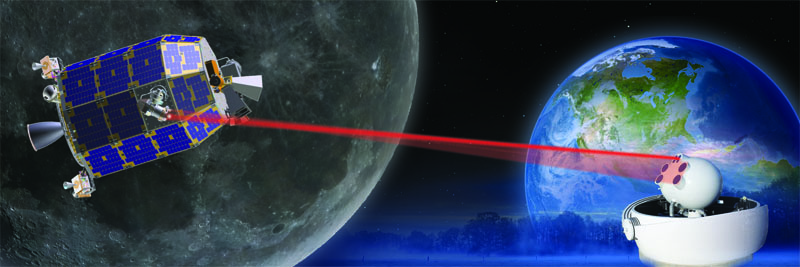
\includegraphics[width=.8\textwidth]{llcd_01} \\
		\end{figure}

		Первый сеанс лазерной связи Земля-Луна состоялся 27 сентября, а 
		теперь LLCD работает на рекордной скорости в 622 мегабит в секунду. 
		Для расстояния в более 380 000 км – это отличный показатель, который 
		в будущем позволит передавать с научных аппаратов огромное количество 
		информации. Прежде всего, удастся увеличить разрешение фотокамер 
		аппаратов и вести передачу 3D-картинки из самых удаленных уголков 
		Солнечной системы.

		Для передачи информации на столь высокой скорости требуется комплекс 
		оптической аппаратуры. Так, на космическом аппарате LADEE установлен 
		приемник с 10-см телескопом и 0,5-ваттный лазерный излучатель, а на 
		наземной станции –- 40-см телескоп. Светочувствительные детекторы 
		обоих приемопередатчиков выполнены по самой современной 
		сверхпроводящей технологии.

		LLCD является кратковременным экспериментом, за которым последует 
		более длительный эксперимент LCRD (Laser Communications Relay 
		Demonstration). Это будет <<репетиция>> последующих 
		миссий, в ходе которых лазерная связь будет основной. Новая технология 
		позволит в ходе миссий, например к Марсу или в Пояс астероидов, 
		собрать во много раз больше ценной научной информации. В более 
		отдаленном будущем высокоскоростные лазерные коммуникации свяжут 
		космические станции, корабли и колонии людей на Луне и Марсе в 
		единую сеть, наподобие интернета.

	\subsection{Технология FSO}
		FSO -- Free Space Optics (WO -- Wireless Optics, АОЛС -- Атмосферная 
		Оптическая Линия Связи) -- вид оптической связи, использующий 
		электромагнитные волны оптического диапазона, передаваемые через 
		атмосферу. В английском языке термин также включает в себя передачу 
		через вакуум.

		В основе беспроводных оптических систем лежат технологии организации 
		высокоскоростных каналов связи посредством инфракрасного излучения, 
		делают возможной передачу данных (текстовые, звуковые, графические 
		данные) между объектами через атмосферное пространство, предоставляя 
		оптическое соединение без использования стекловолокна.

		Лазерная связь двух объектов осуществляется только посредством 
		соединения типа <<точка-точка>>. Технология основывается на передаче 
		данных модулированным излучением в инфракрасной части спектра через 
		атмосферу. Передатчиком служит мощный полупроводниковый лазерный диод. 
		Информация поступает в приемопередающий модуль, в котором кодируется 
		различными помехоустойчивыми кодами, модулируются оптическим лазерным 
		излучателем и фокусируется оптической системой передатчика в узкий 
		коллимированный лазерный луч и передается в атмосферу.

		На принимающей стороне оптическая система фокусирует оптический сигнал 
		на высокочувствительный фотодиод, который преобразует оптический пучок 
		в электрический сигнал. При этом, чем выше частота (до 1,5ГГц), 
		тем больше объём передаваемой информации. Далее, сигнал демодулируется 
		и преобразуется в сигналы выходного интерфейса.

		Длина волны в большинстве реализованных систем варьируется в пределах 
		700—950 нм или 1550 нм, в зависимости от применяемого лазерного диода.

	\section{Типы лазеров}
	\subsection{Полупроводниковые лазеры}
		Принцип действия полупроводниковых лазеров (ППЛ) основан на 
		вынужденной излучательной рекомбинации электронно-дырочных пар, в 
		активных полупроводниковых структурах, получаемых при прохождении 
		через такие структуры электрического тока накачки. 

		Современные ППЛ, применяемые в системах оптической связи, обычно 
		работают в спектральных диапазонах высокой прозрачности кварцевого 
		оптоволокна -- 0.82-0.90 мкм, 1.30-1.33 и около 1.55 мкм. Типичная 
		мощность излучения таких ППЛ от 1 до 5 мВт; увеличение выходной 
		мощности ППЛ сверх 5-10 мВт нецелесообразно, так как срок действия 
		мощных лазеров сравнительно невелик. Кроме этого, при больших 
		плотностях мощности в одномодовом волоке заметную роль начинают 
		играть нелинейно-оптические явления приводящие к искажениям 
		передаваемых сигналов. Ширина спектра излучения лучших образцов 
		промышленных полупроводниковых лазеров около 0.1 нм при уровне 
		боковых частот ниже 20 дБ. В одночастотных ППЛ, используемых в 
		системах когерентной оптической связи, полуширина спектра генерации 
		менее 500 МГц. 

	\subsection{Волоконные лазеры}
		Волоконные лазеры являются одним из наиболее ярких достижений 
		современной квантовой электроники. Это направление возникло на стыке 
		лазерной физики и волоконной оптики. Существует ряд преимуществ 
		волоконных лазеров по сравнению с традиционными квантовыми 
		излучателями, которые позволяют им использоваться наравне с обычными 
		лазерами, а в некоторых случаях и заменить их. Следует отметить, что 
		в начале своего развития основной задачей волоконной оптики 
		представлялось создание волоконных световодов как пассивной среды для 
		передачи информации.

		Понятие <<волоконные лазеры>> охватывает чрезвычайно широкий круг 
		лазерных конфигураций, характеризующихся различными масштабами 
		выходной мощности, а также спектральными и временными характеристиками 
		выходного излучения. 

		Классификация волоконных лазеров по уровням выходной мощности выглядит 
		достаточно условной, отражая в то же время особенности схемы 
		построения лазера. Так, лазеры малой выходной мощности используют 
		накачку в сердцевину световода. Это накладывает ограничения на 
		характеристики полупроводникового источника накачки, который должен 
		иметь характерный размер излучающей области 5 -- 10 мкм. При этом 
		мощность накачки не превышает сотен милливатт, поэтому характерная 
		выходная мощность таких лазеров находится в диапазоне 
		\( 10^{-1} \) -- \( 10^{2} \) мВт.  

		\begin{figure}[!ht]
			\center
			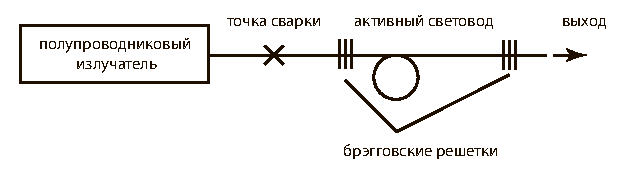
\includegraphics[width=.8\textwidth]{fiber_laser} \\
			\caption{Схематическая установка волоконного лазера}
			\label{img:fiber01}
		\end{figure}

		На рисунке (\ref{img:fiber01}) представлена простейшая конфигурация 
		волоконного лазера с торцевой накачкой, состоящего из 
		полупроводникового источника накачки с волоконным выходом, отрезка 
		волоконного световода, легированного активными ионами, и двух 
		брэгговских решеток. 

		Для накачки активного волоконного световода с двойной оболочкой было 
		предложено несколько способов. Наиболее простым из них является случай 
		торцевой накачки, когда излучение полупроводникового источника 
		вводится в активны световод через торец. Достоинством такого способа 
		является возможность использования для всех видов световодов с 
		двойной оболочкой. К его недостаткам относится возможность 
		использования лишь одного источника накачки (лазерного диода или их 
		сборки), поэтому вводимая в световод мощность ограничена современными 
		возможностями полупроводниковой технологии.

	\subsection{Газовые лазеры}
		Одной из беспроводных технология и является загоризонтная передача 
		информации с помощью лазеров в видимом и инфракрасном диапазонах 
		спектра. При такой передаче не требуется расположение приёмника и 
		источника сигнала в зоне прямой видимости, а используется сигнал, 
		отраженный от атмосферных объектов.

		Система загоризонтной связи позволяет передавать информацию на 
		большие расстояния, не требуя прокладки проводов или оптоволокон, 
		что позволяет сэкономить время и средства. Также можно использовать 
		такую систему в качестве полевой мобильной установки связи при 
		геодезических, геологоразведочных, поисковых, военных и других 
		видах работ, когда требуется связь между несколькими стационарными 
		или подвижными объектами.

		Использование длин волн видимого спектра позволяет упростить настройку 
		такой системы, поскольку оператор может непосредственно видеть 
		точку, сформированную передатчиком, и соответствующим образом 
		настроить приёмник. В свою очередь, использование инфракрасных 
		лазеров может позволить передавать информацию скрытно, при условии, 
		что заранее известна точка, в которую будет направлен луч передатчика.

		В Институте оптики атмосферы им. В.Е. Зуева СО РАН Б.Д. Борисовым был 
		предложен следующий метод передачи информации на основе частотной 
		модуляции излучения лазера на парах бромида меди:
		\begin{itemize}\itemsep-2pt
			\item для передачи информации используются различные расстояни 
				импульсами генерации лазера: <<1>> -- длинная задержка, 
				<<0>> -- короткая задержка;
			\item для обозначения начал передачи используется маркер 
				начала сообщения, отличающийся по длительности от <<0>> и 
				<<1>>;
			\item пакет имеет конечную длину, заранее установленную в 
				интерфейсе (целое число байт);
			\item после передачи полного пакета посылается CRC-сумма, сравнив 
				которую с CRC-суммой полученного сообщения можно однозначно 
				установить, не произошло ли ошибки при передаче;
			\item в случае ошибки, по окончании передачи приёмник повторно 
				запрашивает у передатчика пакет, который был передан с ошибкой.
		\end{itemize}


		Схема управления формирует управляющую последовательность для запуска 
		формирователя высоковольтных импульсов накачки лазера. В качестве 
		приёмника лазерного излучения используется фотодиод.

		\begin{figure}[!ht]
			\center
			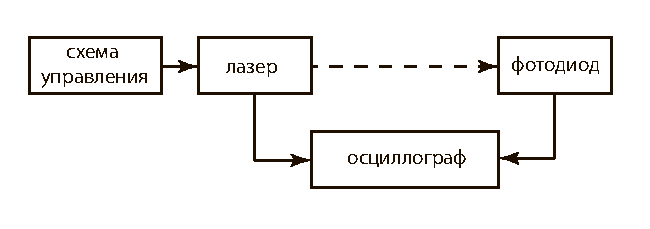
\includegraphics[width=.8\textwidth]{experiment} \\
			\caption{Структурная схема эксперимента}
		\end{figure}

		Недостатком данного метода передачи информации можно считать его 
		метеозависимость, поскольку при отсутствии в атмосфере рассеивающих 
		лазерное излучение объектов передача информации будет практически 
		невозможна.

		Достоинствами являются устойчивость к электромагнитным помехам и 
		возможность широковещательной передачи, т.е. организация системы с 
		одним передатчиком и несколькими приёмниками. По сути, принимать 
		передаваемую информацию можно с любой точки, откуда возможно 
		наблюдать излучение передатчика, рассеянное на атмосферных объектах. 
	
	\pagebreak
	\section{Список используемой литературы}
		\begin{enumerate}\itemsep-2pt
			\item Дмитриев А.Л., Оптические системы передачи информации / 
				учебное пособие. -- СПб: СПбГУИТМО, 2007. -- 96 с.
			\item Васильев А.С., Передача информации с использованием лазера 
				на парах бромида меди / Васильев А.С., Губарев Ф.А., 
				Федоров Ф.В. - Томск.: Томский технический университет 
			\item Курков А.С. Непрерывные волоконные лазеры средней мощности.
				<<Квантовая электроника>>, 34, №10 (2004), 881-900
			\item Википедия -- сводная энциклопедия [Электронный ресурс] // \\
				http://ru.wikipedia.org
		\end{enumerate}
\end{document}